\section{پردازشگر‌های زبان}
\begin{frame}[fragile]{پردازش‌گر‌های زبان}
\begin{itemize}\itemr
\item[-]
به بیان ساده، کامپایلر برنامه‌ایست که می‌تواند یک برنامه را با یک زبان (\lr{\textit{source} language}) بخواند، و معادل آن را به زبانی دیگر ترجمه کند  (\lr{\textit{targer} language}.)
\vspace{6mm}
\begin{figure}[H]
\begin{center}
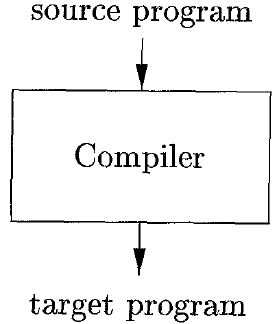
\includegraphics[width=0.3\textwidth, height=0.6\textheight, angle=1]{docs/images/sct}
\end{center}
\end{figure}
\end{itemize}
\end{frame}